\part{Teoretická část}

\chapter{Historie XR}

\section{Počátky XR}

První pokusy o rozšířenou realitu pochází už z 50. let 20. století, kdy Morton Hellig, americký kinematograf, přivádí na svět své zařízení zvané Sensorama. Nejednalo se ovšem o headset, které si vybavíme dnes -- Sensorama bylo stacionární zařízení, vzhledově připomínající automat. Hellig toto zařízení nazýval "zážitkovým divadlem", které bylo schopné zobrazit 3D obraz, pouštět stereo zvuk a vytvářet vítr. Tím se od dnešní XR technologie zásadně liší; nepřijímá vstup uživatele. Sensorama se ovšem nedočkala úspěchu a známe ji jen jako historicky první pokus o virtuální realitu. \cite{otechnice}

Dalším průkopníkem rozšířené reality je Ivan Sutherland, americký vědec, který je často označován jako otec počítačové grafiky. Ve svém díle The Ultimate display (ultimátní displej) popsal virtuální realitu tak, jak ji známe dnes. Virtuální realitu si představoval jako helmu, do které odesílá obraz počítač v reálném čase. Uživatel se tak měl ocitnout ve fiktivním světě nerozpoznatelným od světa reálného. \cite{otechnice} \cite{ivan_sutherland_bio}

Tuto představu se Sutherland snažil realizovat se svými studenty. Společně vynalezli vůbec první headset pro virtuální realitu, zvané The Sword of Damocles -- tedy Damoklův meč. Vzhledem k jeho primitivnosti zobrazovalo pouze čtvercové místnosti tvořené z čar, které software následně transofrmoval do správné perspektivy. Pohyby sledovalo pomocí mechanického ramene připevněného ke stropu, ze kterého byl headset zavěšený. \cite{otechnice} \cite{Rheingold_1992}

\section{XR v armádě}

V 80. letech 20. století o XR projevila zájem armáda USA, ve snaze snadněji a efektivněji připravit americké piloty na ovládání letadel. Začala využívat speciálních simulačních kabin, které obsahovaly mimo jiné i speciální headset. Tento headset pomocí stereoskopického zobrazení informoval o průběhu letu, zobrazoval 3D mapy a snímky z radaru. Díky možnosti systém ovládat pomocí hlasu nebo pohybu očí se tento headset přibližuje k dnešnímu stavu VR, jelikož reaguje na vstup uživatele. \cite{otechnice}


\begin{figure}[H]
    \centering

    \begin{minipage}{.5\textwidth}
        \centering
        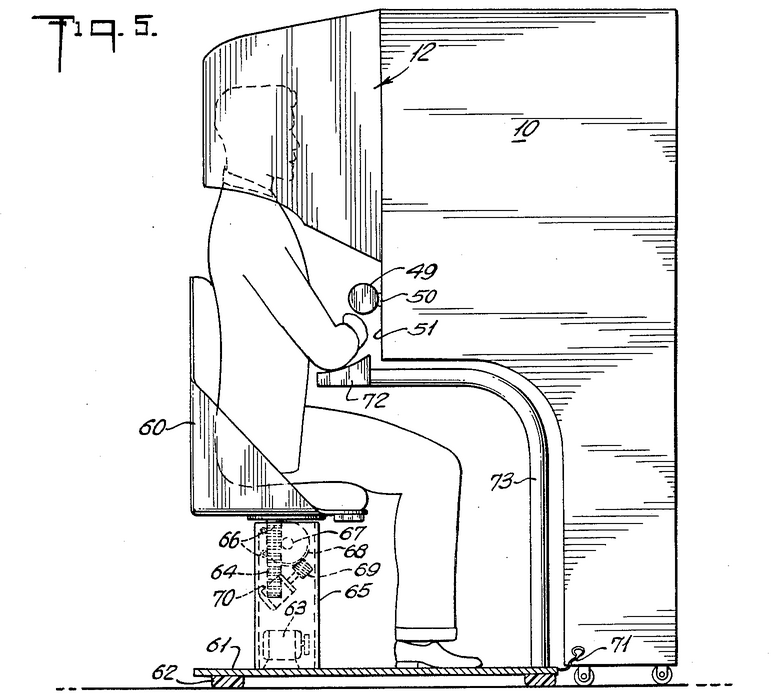
\includegraphics[height=120pt]{sensorama.png}
        \caption{Sensorama \cite{sensorama_patent}}
        \label{sensorama_fig}
    \end{minipage}%
    \begin{minipage}{.5\textwidth}
        \centering
        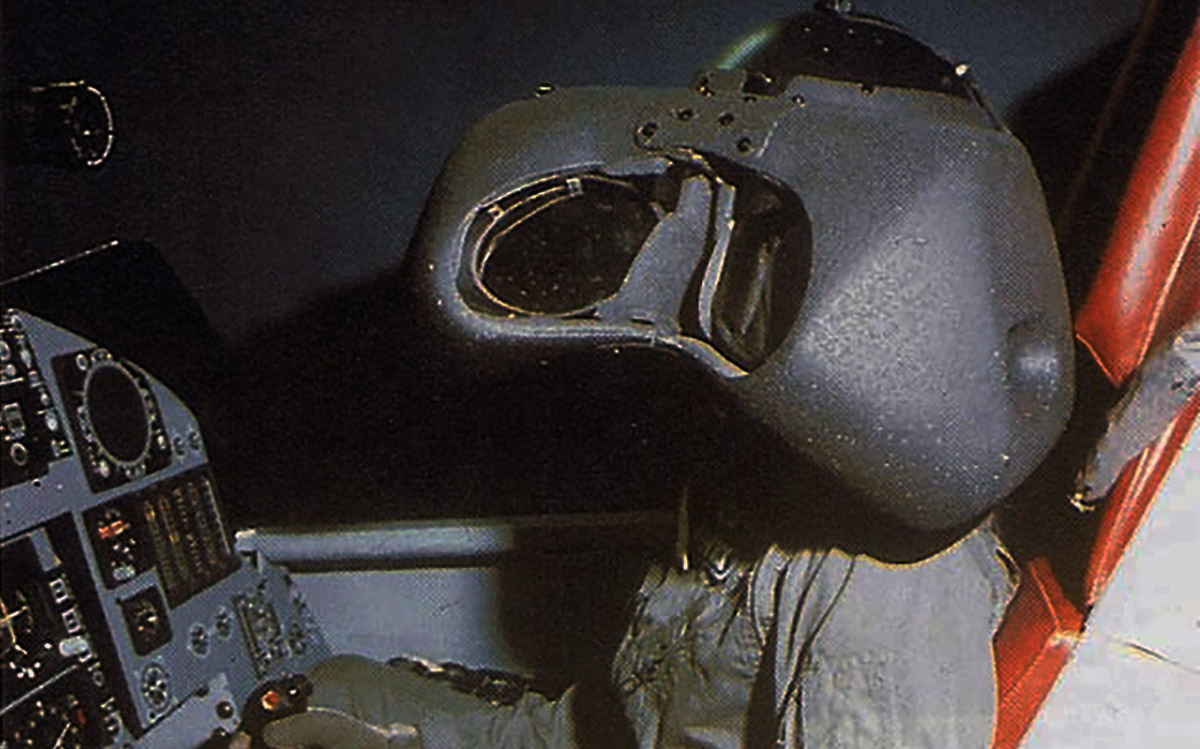
\includegraphics[height=120pt]{super_cockpit_helmet.jpg}
        \caption{Helma "Darth Vader", jedna z částí simulačního kokpitu \cite{super_cockpit_image}}
        \label{sensorama}
    \end{minipage}

\end{figure}

\section{Komerční dostupnost}

\section{XR dnes}

lorem ipsum

\chapter{Hardware}
lorem ipsum

něco o trackování, výrobcích, atd. zmínit trackovací systém bez věží od Meta/FB

rozlišit 6dof vs 3dof

\chapter{Software}
lorem ipsum

zmínit OpenXR, WebXR jakožto API co pohánějí XR

rozlišit PCVR na windows a mobilní VR na bázi androidu